\begin{figure*}
	\begin{subfigure}{5.5cm}
		\centering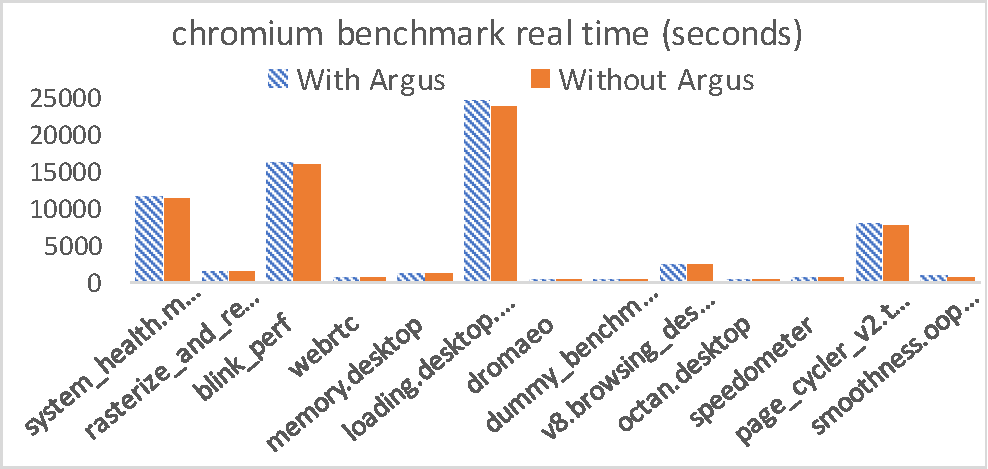
\includegraphics[width = 5cm] {./figures/performance_cr_real.pdf}
		\caption{real time}
	\end{subfigure}
	\begin{subfigure}{5.5cm}
		\centering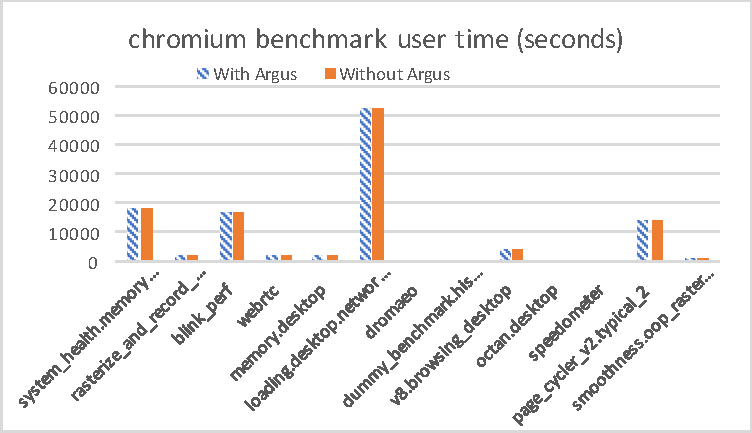
\includegraphics[width = 5cm] {./figures/performance_cr_user.pdf}
		\caption{user time}
	\end{subfigure}
	\begin{subfigure}{5.5cm}
		\centering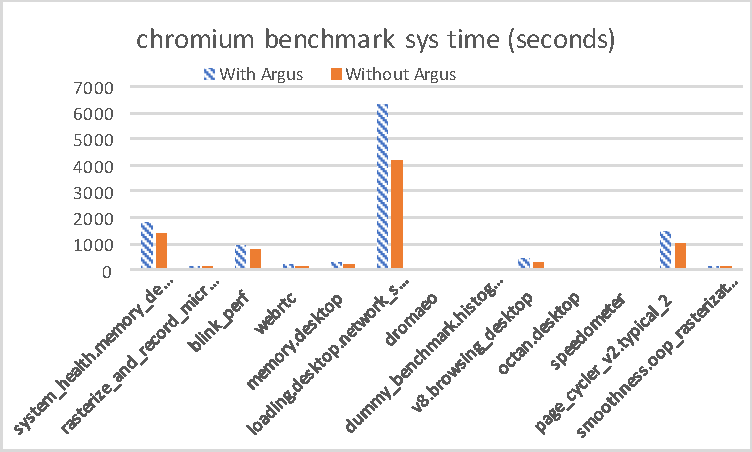
\includegraphics[width = 5cm] {./figures/performance_cr_sys.pdf}
		\caption{sys time}
	\end{subfigure}
	\vspace{-0.5cm}
	\caption{Chromium benchmark}
	\label{fig:chromium benchmark}
\end{figure*}

\begin{table}[tb]
\footnotesize
\centering
\begin{tabularx}{\columnwidth}{l|XXXXX}
\hline
 & 1st & 2nd & 3rd & 4th & 5th\\
\hline\hline
 without \xxx& 5.98 & 6.23 & 6.18 & 6.05 & 6.28\\
 with \xxx& 6.29 & 6.01 & 6.09 & 6.28 & 6.01\\
\hline
average overhead& \multicolumn{5}{c}{0.13\%}\\
\hline
\end{tabularx}
\caption{Score From iBench}
\label{tab:ibench}
\end{table}

\begin{table}[tb]
\footnotesize
\centering
\begin{tabular}{ll|rrr}
\hline
 & kb/s & With Argus & Without Argus & overhead\\
 \hline\hline
\textbf{bonnie++}&read char & 21922 & 22149 & 0.01\\
 sequential& read block & 226931 & 244089 & 0.07\\
 & rewrite & 246807 & 267491 & 0.08\\
 & write char & 22924 & 22936 & 0.00\\
 & write block & 4073361 & 4396387 & 0.07\\
 \hline
 seq& file create & 17391 & 17381 & 0.00\\
 & file delete & 18089 & 19401 & 0.07\\
 \hline
 random& create & 17472 & 17887 & 0.02\\
 & delete & 8849 & 9567 & 0.08\\
 \hline
 \hline
\textbf{iozone} & initial write & 1199453 & 1318572 & 0.09\\
 & rewrite & 3663066 & 4059912 & 0.10\\
 \hline
 & average & - & - & 0.05\\
\hline
\end{tabular}
\caption{IO throughput with bonnie++ and iozone}
\label{tab:iothroughput}
\end{table}


\subsection{Performance Evaluation}\label{sec:evaluation}

In this section we present the performance impact of the live deployment of
\xxx. We deployed \xxx on a MacBookPro9,2, which has Intel Core i5-3210M CPU with
2 cores and 4 thread, 10GB DDR3 memory and a 1T SSD.

\xxx has a very small space overhead with the configuration of its tracing
tool. It uses the ring buffer with configured 2G by default to collect tracing
events. The memory used to store events is fixed to 512M by Apple, which is pretty
low with regards to the memory usage of modern applications. In the remaining
of this section, we measure \xxx's overhead overall with iBench scores, IO
throughput degradation with bonnie++, iozone and CPU overhead with chromium
benchmarks.

\paragraph{iBench}

We first show the five runs of iBench with and without \xxx to evaluate the
overall performance. The machine is clean booted for each run, and the higher
score means it performs better. As shown in Table\ref{tab:ibench}, their
performance are almost of no difference, only 0.13\% degradation on average.

\paragraph{IO Throughput}

Next, we evaluate the IO throughput with bonnie++ and iozone. As shown in the
Table~\ref{tab:iothroughput}, the throughputs of sequential read and write
by characters with and without \xxx are almost same. Read and write by block
impose less than 10\% overhead in  both microbenchmarks, bonni++ and iozone.
With selected events in our system, the tracing tool integrated in \xxx
only adds 5\% IO overhead on average.


\paragraph{CPU}

We evaluate \xxx's CPU overhead with chromium benchmarks by recording their
time usage on real, user and sys. Although the overhead on sys is relatively
higher than other two, due to the tracing events usually crossing the
kernel boundary, they are not triggered too frequently in our daily software
usage, including browsers. The time cost is mostly under 5\%, except the
\vv{dummy\_benchmark.histogram}. As shown in Figure ~\ref{fig:chromium
benchmark}, the time overhead for real, user and sys are 7\%, 5\% and 40\%
respectively.
